\documentclass[10pt]{beamer}

\usetheme{Madrid}
\usecolortheme{default}

% Base packages
\usepackage{amsmath,amssymb,amsthm,mathtools,subcaption,xfrac}
\usepackage{tikz,pgfplots,tabularx,booktabs}
\usetikzlibrary{arrows.meta, positioning, quotes}

\usepackage{xcolor}

% Font settings
\renewcommand{\familydefault}{\sfdefault}

% TikZ libraries
\usetikzlibrary{calc,positioning,backgrounds,decorations.pathreplacing}
\pgfplotsset{compat=1.14}

% Colors
\definecolor{deepblue}{RGB}{42,39,155}
\definecolor{lightpink}{RGB}{255,240,240}
\definecolor{lightgreen}{RGB}{240,255,240}
\definecolor{lightyellow}{RGB}{255,255,240}
\definecolor{codegray}{RGB}{245,245,245}
\definecolor{codegreen}{rgb}{0,0.6,0}
\definecolor{codepurple}{rgb}{0.58,0,0.82}

% Beamer settings
\setbeamercolor{title}{fg=white,bg=deepblue}
\setbeamercolor{frametitle}{fg=white,bg=deepblue}
\setbeamercolor{section in head/foot}{fg=white,bg=deepblue}

\setbeamertemplate{footline}[text line]{%
  \parbox{\linewidth}{\vspace*{-8pt}
    \hfill
    \insertframenumber~/ \inserttotalframenumber}}
\setbeamertemplate{navigation symbols}{}

\definecolor{foo}{rgb}{.2,.2,.7}
\AtBeginSection[]{
  \begin{frame}
  \vfill
  \centering
  \begin{beamercolorbox}[sep=8pt,center,shadow=true,rounded=true]{section page}
    \usebeamerfont{title}%
    {\color{foo} \insertsectionhead}\par%
  \end{beamercolorbox}
  \vfill
  \end{frame}
}

\DeclareMathOperator\prb{\mathsf{P}}
\DeclareMathOperator\expc{\mathsf{E}}
\DeclareMathOperator\var{var}
\DeclareMathOperator\cov{cov}
\DeclareMathOperator\cor{corr}
\DeclareMathOperator*{\argmax}{\arg\!\max}
\DeclareMathOperator*{\argmin}{\arg\!\min}
\DeclareMathOperator\corr{corr}
\DeclareMathOperator\rk{rank}
\DeclareMathOperator\sgn{sgn}
\DeclareMathOperator{\tr}{tr}

% Blackboard bold
\renewcommand{\AA}{\mathbb A}
\newcommand{\CC}{\mathbb C}
\newcommand{\DD}{\mathbb D}
\newcommand{\EE}{\mathbb E}
\newcommand{\FF}{\mathbb F}
\newcommand{\HH}{\mathbb H}
\newcommand{\KK}{\mathbb K}
\newcommand{\NN}{\mathbb N}
\newcommand{\PP}{\mathbb P}
\newcommand{\QQ}{\mathbb Q}
\newcommand{\RR}{\mathbb R}
\newcommand{\UU}{\mathbb U}
\newcommand{\ZZ}{\mathbb Z}

\newcommand{\ie}{\;\Longrightarrow\;}
\newcommand{\ifff}{\;\Longleftrightarrow\;}
\newcommand{\ds}{\displaystyle}

\title{Financial Markets \& Instruments}
\author{}
\date{}

\begin{document}

\begin{frame}
\titlepage
\end{frame}

\begin{frame}{What is Finance?}
  \begin{itemize}[<+->]
    \item A possible definition:
    \begin{quote}
      Finance is the study of how people and organizations allocate scarce resources over time, subject to uncertainty.
    \end{quote}
    \item Two essential ingredients:
      \begin{itemize}
        \item \textbf{Time}: Reflected in interest rates, borrowing, and investing
        \item \textbf{Uncertainty}: Future asset values, returns, and economic conditions
      \end{itemize}
    \item These two dimensions are intertwined throughout all financial concepts and models
    \item Financial markets facilitate:
      \begin{itemize}
        \item Consumption timing (saving and borrowing)
        \item Risk transfer between market participants
      \end{itemize}
  \end{itemize}
\end{frame}

\begin{frame}{Consumption Timing}
  \begin{itemize}[<+->]
    \item Imagine a world without ``storage'' of money: 
      \begin{itemize}
        \item We would have to consume all income immediately
        \item No saving for future needs, no borrowing against future income
      \end{itemize}
    \item Financial markets allow shifting consumption across time
      \begin{itemize}
        \item Money markets: Short-term borrowing and lending
        \item Capital markets: Long-term investment and financing
      \end{itemize}
    \item Time value of money: $\$1$ now is worth more than $\$1$ in the future
      \begin{itemize}
        \item Investment opportunities
        \item Precautionary cushion against unforeseen needs
      \end{itemize}
    \item Shifting consumption comes with compensation in the form of interest rates
  \end{itemize}
\end{frame}

\begin{frame}{Shifting Consumption in Time}
\begin{figure}
  \centering
  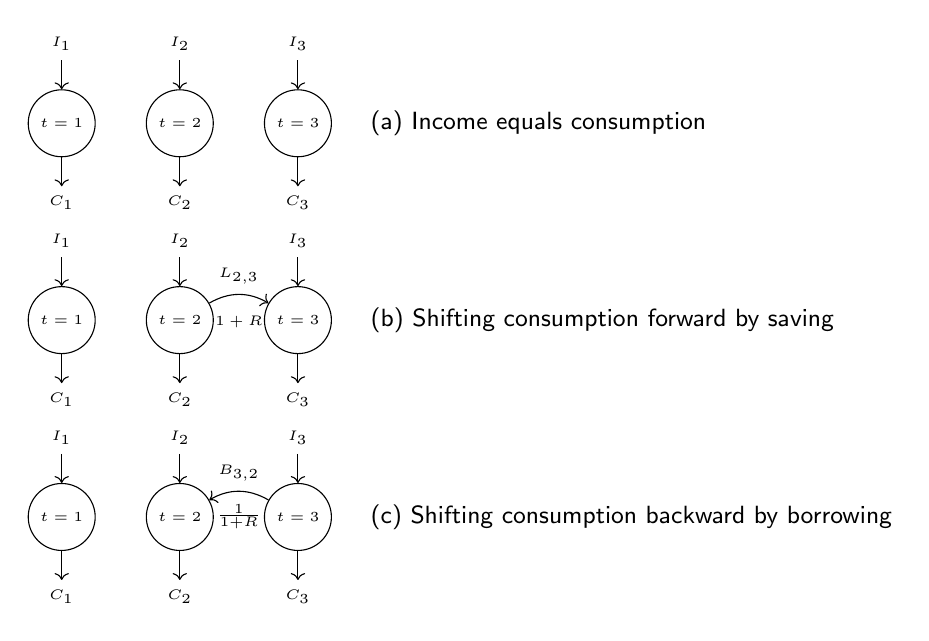
\begin{tikzpicture}[scale=1]
    % First diagram (Income equals consumption)
    \node[circle,draw,font=\tiny] (t1a) at (0,0) {$t=1$};
    \node[circle,draw,font=\tiny] (t2a) at (1.5,0) {$t=2$};
    \node[circle,draw,font=\tiny] (t3a) at (3,0) {$t=3$};
    
    \draw[->] (0,0.8) node[above,font=\tiny]{$I_1$} -- (t1a);
    \draw[->] (1.5,0.8) node[above,font=\tiny]{$I_2$} -- (t2a);
    \draw[->] (3,0.8) node[above,font=\tiny]{$I_3$} -- (t3a);
    
    \draw[->] (t1a) -- (0,-0.8) node[below,font=\tiny]{$C_1$};
    \draw[->] (t2a) -- (1.5,-0.8) node[below,font=\tiny]{$C_2$};
    \draw[->] (t3a) -- (3,-0.8) node[below,font=\tiny]{$C_3$};
    
    % Label to the right
    \node[right,font=\small] at (3.8,0) {(a) Income equals consumption};
    
    % Second diagram (Shifting consumption forward) - 2.5 units down
    \node[circle,draw,font=\tiny] (t1b) at (0,-2.5) {$t=1$};
    \node[circle,draw,font=\tiny] (t2b) at (1.5,-2.5) {$t=2$};
    \node[circle,draw,font=\tiny] (t3b) at (3,-2.5) {$t=3$};
    
    \draw[->] (0,-1.7) node[above,font=\tiny]{$I_1$} -- (t1b);
    \draw[->] (1.5,-1.7) node[above,font=\tiny]{$I_2$} -- (t2b);
    \draw[->] (3,-1.7) node[above,font=\tiny]{$I_3$} -- (t3b);
    
    \draw[->] (t1b) -- (0,-3.3) node[below,font=\tiny]{$C_1$};
    \draw[->] (t2b) -- (1.5,-3.3) node[below,font=\tiny]{$C_2$};
    \draw[->] (t3b) -- (3,-3.3) node[below,font=\tiny]{$C_3$};
    
    \draw[->] (t2b) to[bend left] node[above,font=\tiny]{$L_{2,3}$} (t3b);
    \node[below,font=\tiny] at (2.25,-2.32) {$1+R$};
    
    % Label to the right
    \node[right,font=\small] at (3.8,-2.5) {(b) Shifting consumption forward by saving};
    
    % Third diagram (Shifting consumption backward) - 5 units down
    \node[circle,draw,font=\tiny] (t1c) at (0,-5) {$t=1$};
    \node[circle,draw,font=\tiny] (t2c) at (1.5,-5) {$t=2$};
    \node[circle,draw,font=\tiny] (t3c) at (3,-5) {$t=3$};
    
    \draw[->] (0,-4.2) node[above,font=\tiny]{$I_1$} -- (t1c);
    \draw[->] (1.5,-4.2) node[above,font=\tiny]{$I_2$} -- (t2c);
    \draw[->] (3,-4.2) node[above,font=\tiny]{$I_3$} -- (t3c);
    
    \draw[->] (t1c) -- (0,-5.8) node[below,font=\tiny]{$C_1$};
    \draw[->] (t2c) -- (1.5,-5.8) node[below,font=\tiny]{$C_2$};
    \draw[->] (t3c) -- (3,-5.8) node[below,font=\tiny]{$C_3$};
    
    \draw[->] (t3c) to[bend right] node[above,font=\tiny]{$B_{3,2}$} (t2c);
    \node[below,font=\tiny] at (2.25,-4.72) {$\tfrac{1}{1+R}$};
    
    % Label to the right
    \node[right,font=\small] at (3.8,-5) {(c) Shifting consumption backward by borrowing};
  \end{tikzpicture}
  \caption{Shifting consumption forward and backward in time}
\end{figure}
\end{frame}

\begin{frame}{Flow Balance Equations}
  \begin{itemize}[<+->]
    \item When saving (shifting consumption forward):
      \begin{align*}
        C_2 &= I_2 - L_{2,3} \\
        C_3 &= I_3 + L_{2,3}(1 + R)
      \end{align*}
      where $L_{2,3}$ is the amount saved/lent and $R$ is the interest rate
    \item When borrowing (shifting consumption backward):
      \begin{align*}
        C_2 &= I_2 + \tfrac{B_{3,2}}{1 + R} \\
        C_3 &= I_3 - B_{3,2}
      \end{align*}
      where $B_{3,2}$ is the amount to be repaid at $t=3$
    \item Alternative expression when borrowing at $t=2$:
      \begin{align*}
        C_2 &= I_2 + B^*_{3,2} \\
        C_3 &= I_3 - B^*_{3,2}(1 + R)
      \end{align*}
      where $B^*_{3,2}$ is the amount borrowed at $t=2$
  \end{itemize}
\end{frame}

\begin{frame}{Uncertainty and Risk}
  \begin{itemize}[<+->]
    \item Financial markets not only deal with time, but also uncertainty
    \item Sources of financial risk:
      \begin{itemize}
        \item Market risk: Fluctuations in stock prices, interest rates, etc.
        \item Credit risk: Possibility of default on debt obligations
        \item Currency risk: Exchange rate fluctuations
        \item Inflation risk: Loss of purchasing power
        \item Operational risk: Failures in processes, systems, or people
      \end{itemize}
    \item Risk vs. uncertainty: Risk can be quantified with probabilities
    \item Risk transfer: Insurance markets, derivatives markets
    \item Risk management: Identifying, measuring, and controlling risk exposures
  \end{itemize}
\end{frame}

%\begin{frame}{Representing Uncertainty}
%  \begin{figure}
%    \centering
%    \begin{tikzpicture}[scale=0.6]
%      % Current state
%      \node[circle,draw] (t0) at (0,0) {};
%      
%      % Future states
%      \node[circle,draw] (w1) at (6,4) {$\omega_1$};
%      \node[circle,draw] (w2) at (6,2) {$\omega_2$};
%      \node[circle,draw] (w3) at (6,0) {$\omega_3$};
%      \node[circle,draw] (w4) at (6,-2) {$\omega_4$};
%      \node[circle,draw] (w5) at (6,-4) {$\omega_5$};
%      
%      % Connections
%      \draw[->] (t0) -- (w1) node[midway,above,sloped] {$\pi_1$};
%      \draw[->] (t0) -- (w2) node[midway,above,sloped] {$\pi_2$};
%      \draw[->] (t0) -- (w3) node[midway,above,sloped] {$\pi_3$};
%      \draw[->] (t0) -- (w4) node[midway,above,sloped] {$\pi_4$};
%      \draw[->] (t0) -- (w5) node[midway,above,sloped] {$\pi_5$};
%      
%      % Time labels
%      \node at (0,-6) {$t = 0$};
%      \node at (6,-6) {$t = T$};
%    \end{tikzpicture}
%    \caption{Representing uncertain states of the world by a scenario fan}
%  \end{figure}
%\end{frame}

\begin{frame}{Holding Period Return and Gain}
  \begin{itemize}[<+->]
    \item \textbf{Definition 1.1 (Holding period return)} Let us consider a holding period $[0, T]$, where the initial asset price is $S(0)$ and the terminal random asset price is $S(T, \omega)$. We define the holding period return as
    \begin{align*}
      R(\omega) \doteq \tfrac{S(T, \omega) - S(0)}{S(0)}
    \end{align*}
    and the holding period gain as
    \begin{align*}
      G(\omega) \doteq \tfrac{S(T, \omega)}{S(0)} = 1 + R(\omega)
    \end{align*}
    \item A return of 10\% means the stock price was multiplied by a gain factor of 1.10
    \item Gain (or gross return) vs. return (or net return)
    \item Term ``rate of return'' typically reserved for annual returns
  \end{itemize}
\end{frame}

\begin{frame}{Different Types of Returns}
  \begin{itemize}[<+->]
    \item Consider a holding period of two consecutive years:
    \begin{itemize}
      \item Year 1: Return is +10\%
      \item Year 2: Return is -10\%
      \item What is the ``average'' return?
    \end{itemize}
    \item Arithmetic mean: $R_a = \tfrac{0.10 + (-0.10)}{2} = 0$
    \item But actual gain over two years:
    \begin{align*}
      G &= (1 + 0.10) \times (1 - 0.10) \\
      &= 0.99 \quad \text{(a loss of 1\%)}
    \end{align*}
    \item Geometric average (annualized): 
    \begin{align*}
      (1 + 0.10) \times (1 - 0.10) &= (1 + R_g)^2 \\
      \Rightarrow R_g &= -0.5013\%
    \end{align*}
    \item The return depends on the measurement approach
  \end{itemize}
\end{frame}

%\begin{frame}{Normal vs. Lognormal Distributions}
%  \begin{itemize}[<+->]
%    \item Can we model stock returns with a normal distribution?
%      \begin{itemize}
%        \item Empirical evidence shows returns have ``fat tails'' (more extreme events)
%        \item Normal distribution has thin tails and unlimited range
%        \item Stock returns cannot be less than -100\% (limited liability)
%      \end{itemize}
%    \item Cross-sectional perspective (portfolio of stocks):
%      \begin{itemize}
%        \item If individual returns $R_a$ and $R_b$ are normal, portfolio return $R_p = 0.3R_a + 0.7R_b$ is also normal
%        \item Convenient for portfolio theory
%      \end{itemize}
%    \item Longitudinal perspective (one stock over time):
%      \begin{itemize}
%        \item For consecutive periods, gains multiply: $G = G(1) \times G(2)$
%        \item This gives $1 + R = (1 + R(1))(1 + R(2)) = 1 + R(1) + R(2) + R(1)R(2)$
%        \item Product term breaks normality
%      \end{itemize}
%  \end{itemize}
%\end{frame}
%
%\begin{frame}{Log-Returns}
%  \begin{itemize}[<+->]
%    \item Log-return (continuously compounded return):
%    \begin{align*}
%      r \doteq \log(1 + R) \equiv \log G
%    \end{align*}
%    \item For small $x$, $\log(1 + x) \approx x$, so log-returns approximate standard returns
%    \item Multi-period additivity:
%    \begin{align*}
%      \log\left[(1 + R(1))(1 + R(2))\right] &= \log(1 + R(1)) + \log(1 + R(2))\\
%      &= r(1) + r(2)
%    \end{align*}
%    \item If log-returns are normal, gains are lognormal:
%    \begin{align*}
%      S(T) = S(0) \cdot G = S(0) \cdot e^r
%    \end{align*}
%    \item Tradeoffs:
%      \begin{itemize}
%        \item Normal returns: Good for portfolios, problematic for multi-period
%        \item Lognormal returns: Stock prices always positive, good for multi-period, complicates portfolio analysis
%      \end{itemize}
%  \end{itemize}
%\end{frame}

\begin{frame}{Risk-Free Asset}
  \begin{itemize}[<+->]
    \item A risk-free asset has a predetermined return with certainty
    \item Example: Safe bank account or high-quality government bonds
    \item For a risk-free asset:
    \begin{align*}
      B(T, \omega) = B(0) \cdot (1 + R_f)
    \end{align*}
    for every state of the world $\omega \in \Omega$
    \item $R_f$ is the risk-free return; if $T$ is one year, referred to as risk-free rate
    \item Why invest in risky assets if risk-free ones exist?
      \begin{itemize}
        \item Risk premium: Compensation for bearing risk
        \item Higher expected returns for risky assets
      \end{itemize}
    \item Risky and risk-free assets form the foundation of many financial models
  \end{itemize}
\end{frame}

\begin{frame}{Market Scenario Trees}
\begin{figure}
  \centering
  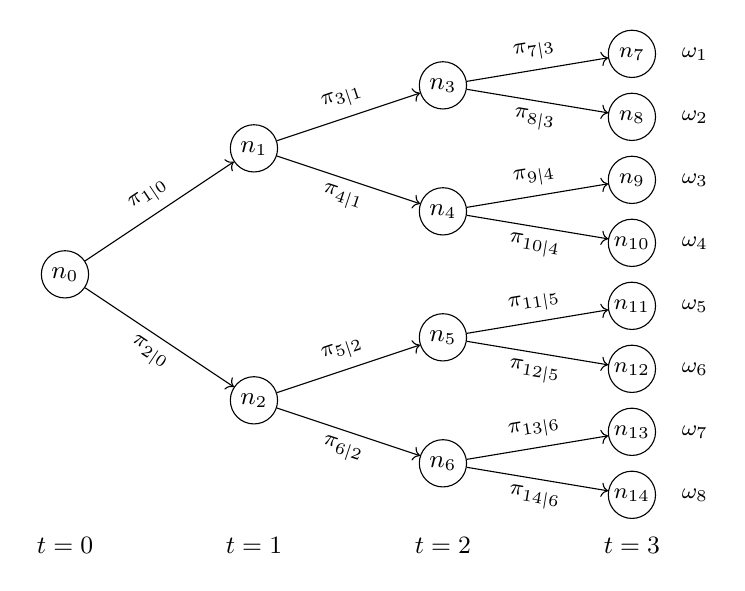
\begin{tikzpicture}[
    scale=0.8, 
    every node/.style={font=\small},
    circ/.style={circle,draw,minimum size=0.6cm,inner sep=1pt}
  ]
    % Root node
    \node[circ] (n0) at (0,0) {$n_0$};
    
    % Level 1 nodes
    \node[circ] (n1) at (3,2) {$n_1$};
    \node[circ] (n2) at (3,-2) {$n_2$};
    
    % Level 2 nodes
    \node[circ] (n3) at (6,3) {$n_3$};
    \node[circ] (n4) at (6,1) {$n_4$};
    \node[circ] (n5) at (6,-1) {$n_5$};
    \node[circ] (n6) at (6,-3) {$n_6$};
    
    % Level 3 nodes
    \node[circ,font=\footnotesize] (n7) at (9,3.5) {$n_7$};
    \node[circ,font=\footnotesize] (n8) at (9,2.5) {$n_8$};
    \node[circ,font=\footnotesize] (n9) at (9,1.5) {$n_9$};
    \node[circ,font=\footnotesize] (n10) at (9,0.5) {$n_{10}$};
    \node[circ,font=\footnotesize] (n11) at (9,-0.5) {$n_{11}$};
    \node[circ,font=\footnotesize] (n12) at (9,-1.5) {$n_{12}$};
    \node[circ,font=\footnotesize] (n13) at (9,-2.5) {$n_{13}$};
    \node[circ,font=\footnotesize] (n14) at (9,-3.5) {$n_{14}$};
    
    % Connections
    \draw[->] (n0) -- (n1) node[midway,above,sloped,font=\footnotesize] {$\pi_{1|0}$};
    \draw[->] (n0) -- (n2) node[midway,below,sloped,font=\footnotesize] {$\pi_{2|0}$};
    
    \draw[->] (n1) -- (n3) node[midway,above,sloped,font=\footnotesize] {$\pi_{3|1}$};
    \draw[->] (n1) -- (n4) node[midway,below,sloped,font=\footnotesize] {$\pi_{4|1}$};
    \draw[->] (n2) -- (n5) node[midway,above,sloped,font=\footnotesize] {$\pi_{5|2}$};
    \draw[->] (n2) -- (n6) node[midway,below,sloped,font=\footnotesize] {$\pi_{6|2}$};
    
    \draw[->] (n3) -- (n7) node[midway,above,sloped,font=\footnotesize] {$\pi_{7|3}$};
    \draw[->] (n3) -- (n8) node[midway,below,sloped,font=\footnotesize] {$\pi_{8|3}$};
    \draw[->] (n4) -- (n9) node[midway,above,sloped,font=\footnotesize] {$\pi_{9|4}$};
    \draw[->] (n4) -- (n10) node[midway,below,sloped,font=\footnotesize] {$\pi_{10|4}$};
    \draw[->] (n5) -- (n11) node[midway,above,sloped,font=\footnotesize] {$\pi_{11|5}$};
    \draw[->] (n5) -- (n12) node[midway,below,sloped,font=\footnotesize] {$\pi_{12|5}$};
    \draw[->] (n6) -- (n13) node[midway,above,sloped,font=\footnotesize] {$\pi_{13|6}$};
    \draw[->] (n6) -- (n14) node[midway,below,sloped,font=\footnotesize] {$\pi_{14|6}$};
    
    % Time labels
    \node at (0,-4.3) {$t = 0$};
    \node at (3,-4.3) {$t = 1$};
    \node at (6,-4.3) {$t = 2$};
    \node at (9,-4.3) {$t = 3$};
    
    % Scenario labels
    \node[font=\footnotesize] at (10,3.5) {$\omega_1$};
    \node[font=\footnotesize] at (10,2.5) {$\omega_2$};
    \node[font=\footnotesize] at (10,1.5) {$\omega_3$};
    \node[font=\footnotesize] at (10,0.5) {$\omega_4$};
    \node[font=\footnotesize] at (10,-0.5) {$\omega_5$};
    \node[font=\footnotesize] at (10,-1.5) {$\omega_6$};
    \node[font=\footnotesize] at (10,-2.5) {$\omega_7$};
    \node[font=\footnotesize] at (10,-3.5) {$\omega_8$};
  \end{tikzpicture}
  \caption{A scenario tree: uncertainty unfolding progressively over time}
\end{figure}
\end{frame}


\begin{frame}{Types of Assets}
  \begin{itemize}[<+->]
    \item An \textbf{asset} is anything that can be transformed into money by its owner
    \item Key dimensions for classifying assets:
      \begin{itemize}
        \item \textbf{Real vs. financial}: Physical assets vs. securities/claims
        \item \textbf{Risky vs. risk-free}: Uncertain vs. certain future value
        \item \textbf{Liquid vs. illiquid}: Ease of selling at fair price
        \item \textbf{Tradable vs. non-tradable}: Can be bought/sold in markets
        \item \textbf{Exchange-traded vs. over-the-counter (OTC)}: Standardized vs. customized
      \end{itemize}
    \item Main types of financial assets:
      \begin{itemize}
        \item Stock shares (equity)
        \item Bonds and other debt securities
        \item Foreign currencies
        \item Derivatives: Forwards/futures, options, swaps
        \item Hybrid securities
      \end{itemize}
  \end{itemize}
\end{frame}

\begin{frame}{Assets vs. Securities}
  \begin{itemize}[<+->]
    \item \textbf{Securities} are tradable financial assets
      \begin{itemize}
        \item Readily purchased or sold on financial markets
        \item Examples: Stocks, bonds, exchange-traded derivatives
      \end{itemize}
    \item Not all assets are securities:
      \begin{itemize}
        \item Insurance policies: Assets but not tradable
        \item Human capital: Valuable but not marketable
        \item Bank loans: Assets for the bank but not readily tradable
      \end{itemize}
    \item \textbf{Securitization}: Transforming illiquid assets into tradable securities
      \begin{itemize}
        \item Example: Mortgages → Mortgage-backed securities (MBS)
        \item Pools cash flows from similar assets
        \item Creates liquid securities from illiquid assets
      \end{itemize}
    \item Liquidity depends on both asset type and market conditions
  \end{itemize}
\end{frame}

\begin{frame}{Equity}
  \begin{itemize}[<+->]
    \item Stock shares represent residual claims on the equity of a firm
      \begin{itemize}
        \item If a firm is liquidated, assets are sold to pay liabilities
        \item Any remaining equity is distributed to stockholders
        \item This is why stocks are referred to as ``equity'' investments
      \end{itemize}
    \item Holding period return for a stock share: $\ds R(\omega) = \tfrac{S(T, \omega) + D - S(0)}{S(0)}$ where $D$ is dividend paid during the holding period $(0, T)$
      \begin{itemize}
        \item Dividend timing affects valuation when reinvested
        \item Forward-projected dividends should be considered in calculations
      \end{itemize}
    \item Key features of stock shares:
      \begin{itemize}
        \item Limited liability assets: stockholders not responsible for firm's illegal behavior
        \item Stock prices cannot be negative and worst-case return is $-100\%$
        \item Common vs. preferred stock shares with different voting rights and dividend guarantees
        \item No defined maturity, unlike bonds or options
        \item Stock shares can be created and destroyed (unlike energy in physics)
      \end{itemize}
    \item Extraordinary events affecting stock prices:
      \begin{itemize}
        \item Stock splits and reverse splits: create multiple shares from one or vice versa
        \item Spinoffs: firm separates into two with corresponding shares
        \item Mergers and acquisitions: firms combine with share conversion
        \item These events affect price but not market capitalization
      \end{itemize}
  \end{itemize}
\end{frame}

\begin{frame}{Fixed Income}
  \begin{itemize}[<+->]
    \item A bond is a security defined by:
      \begin{itemize}
        \item Face value $F$ (nominal or par value): amount issuer promises to pay
        \item Maturity $T$ (time when face value is paid back)
        \item Coupon rate $c$ (interest rate applied to face value for periodic payments)
        \item Coupons historically were physical pieces of paper detached for payment
      \end{itemize}
    \item Types of bonds:
      \begin{itemize}
        \item Zero-coupon bonds ($c = 0$): no periodic payments, only face value at maturity
        \item Coupon-bearing bonds ($c > 0$): periodic interest payments plus face value
        \item Coupon frequency typically twice a year, but can vary
      \end{itemize}
    \item US Treasury bonds classified as:
      \begin{itemize}
        \item T-bills: zeros, maturities up to one year
        \item T-notes: coupon-bearing, maturities up to ten years
        \item T-bonds: coupon-bearing, longer maturities
        \item Some long-term zeros created by stripping coupons (unbundling cash flows)
      \end{itemize}
    \item Bond risk factors:
      \begin{itemize}
        \item Default risk: issuer may fail to pay coupons or principal
        \item Inflation risk: relevant for long-term bonds, erodes purchasing power
        \item Foreign-exchange risk: for bonds denominated in foreign currencies
        \item Interest rate risk: inverse relationship between rates and bond prices
      \end{itemize}
  \end{itemize}
\end{frame}

\begin{frame}{FOREX Markets}
  \begin{itemize}[<+->]
    \item Foreign exchange (FOREX) markets facilitate currency trading
      \begin{itemize}
        %\item One of the largest global markets by trading volume
        \item Important for international equity and fixed-income portfolios
        \item Also critical for non-financial firms with international operations
      \end{itemize}
    \item Risk factor: exchange rate between currency pairs
      \begin{itemize}
        \item Affects international trade and investments
        \item Source of both risk and speculative opportunity
      \end{itemize}
    \item Quotation conventions:
      \begin{itemize}
        \item Currency pair notation (e.g., EUR/USD = 1.1166)
        \item Base currency (left of slash): fixed amount (e.g., EUR 1)
        \item Quoted currency (right of slash): variable amount (e.g., USD 1.1166)
        \item Means 1 euro can buy 1.1166 US dollars
      \end{itemize}
    \item Direct vs. indirect quotation:
      \begin{itemize}
        \item Direct: domestic currency is quoted currency (variable amount)
        \item Indirect: domestic currency is base currency (fixed amount)
        \item Also called ``uncertain for certain'' vs. ``certain for uncertain''
        \item Choice depends on perspective, convenience, and local conventions
      \end{itemize}
    \item Bid-ask spreads: difference between buying and selling prices
      \begin{itemize}
        \item Example: EUR/USD 1.1165/67
        \item Bank buys base currency (EUR) at bid price (1.1165)
        \item Bank sells base currency at ask price (1.1167)
        \item ``Three Bs rule'': market maker Buys the Base currency at the Bid price
      \end{itemize}
  \end{itemize}
\end{frame}

\begin{frame}{Derivatives}
  \begin{itemize}[<+->]
    \item Derivative: financial asset deriving its value from an underlying variable
      \begin{itemize}
        \item Defined by explicit formula written in contract
        \item Typical payoff is $f(S_T)$ for some function $f(\cdot)$ at maturity $T$
        \item More complex derivatives depend on price path until maturity
      \end{itemize}
    \item Types of underlying variables:
      \begin{itemize}
        \item Primary financial assets (stocks, bonds)
        \item Nonfinancial assets (commodities like gold or oil)
        \item Risk factors (interest rates, market indexes, volatility)
        \item Weather or other non-price variables
        \item Other derivatives (compound options, swaptions)
      \end{itemize}
    \item Key issues in derivatives:
      \begin{itemize}
        \item Pricing: determining fair value based on underlying factors
        \item Hedging: managing risk exposure of writing derivatives
        \item Portfolio management: changing exposure to risk factors
        \item Regulatory and accounting issues beyond scope of quantitative models
      \end{itemize}
    \item Basic derivative families:
      \begin{itemize}
        \item Forward contracts: obligation to buy/sell at future date
        \item Futures contracts: standardized, exchange-traded forwards
        \item Options: right but not obligation to buy/sell
        \item Plain vanilla vs. exotic derivatives with complex payoffs
      \end{itemize}
  \end{itemize}
\end{frame}

\begin{frame}{Forward Contracts}
  \begin{itemize}[<+->]
    \item Agreement between two counterparties to buy/sell an asset at a prespecified forward price $F(t_0, T)$ at a later date $T$
      \begin{itemize}
        \item A private arrangement between counterparties (OTC)
        \item Both parties are obligated to fulfill the contract terms
      \end{itemize}
    \item Long position: agrees to buy the asset at maturity
    \item Short position: agrees to sell the asset at maturity
    \item At maturity, spot-forward convergence applies: $S(T) = F(T, T)$
      \begin{itemize}
        \item Forward price at maturity equals spot price (law of one price)
        \item Otherwise would create arbitrage opportunity
      \end{itemize}
    \item Payoff for long position: $S(T) - F(t_0, T)$
      \begin{itemize}
        \item Positive when spot price exceeds delivery price
        \item Negative when delivery price exceeds spot price
      \end{itemize}
    \item Payoff for short position: $F(t_0, T) - S(T)$
      \begin{itemize}
        \item Zero-sum game: one party's gain is other's loss
      \end{itemize}
    \item Forward contracts:
      \begin{itemize}
        \item Tailored to specific needs (OTC)
        \item Less liquid and standardized than futures
        \item Subject to counterparty risk (default risk)
        \item Initial value is zero, allowing leverage without initial investment
        \item Used for both hedging and speculation
      \end{itemize}
  \end{itemize}
\end{frame}

\begin{frame}{Futures Contracts}
  \begin{itemize}[<+->]
    \item Exchange-traded equivalents of forward contracts
      \begin{itemize}
        %\item Similar in concept but with important institutional differences
        \item Delivery of underlying or cash settlement at maturity
      \end{itemize}
    \item Key features to address issues with forwards:
      \begin{itemize}
        %\item Standardization to improve liquidity
        \item Clearinghouse to reduce counterparty risk
        \item Daily marking-to-market instead of single settlement
      \end{itemize}
    \item Standardization:
      \begin{itemize}
        \item Limited underlying assets and delivery dates
        \item Deep market with easier entry/exit
        \item Standard contract sizes (e.g., 100 oz gold)
        \item Sometimes allows range of deliverable assets (e.g., bond futures)
      \end{itemize}
    \item Clearinghouse:
      \begin{itemize}
        \item Steps between long and short positions as counterparty
        \item Assumes counterparty risk from both sides
        \item Manages margin accounts for all positions
        \item Nets positions to reduce exposure (proved effective in 1987 crash)
      \end{itemize}
    \item Daily marking-to-market:
      \begin{itemize}
        \item Daily cash flow settlements based on price changes
        \item Margin accounts with initial and maintenance margins
        \item Margin calls when account drops below threshold
        \item Position liquidated if margin call not met
        \item Sum of daily cash flows equals forward contract payoff
      \end{itemize}
  \end{itemize}
\end{frame}

\begin{frame}{Vanilla Options I}
  \begin{itemize}[<+->]
    \item Asymmetric contracts with nonlinear payoffs
      \begin{itemize}
        \item Two distinct roles: option writer and option holder
        \item Option writer creates and sells the option
        \item Option holder purchases the right but not obligation
      \end{itemize}
    \item Call option: right (not obligation) to buy the underlying asset at strike price $K$
      \begin{itemize}
        \item Profitable when asset price exceeds strike price
        \item Maximum loss limited to premium paid
        \item Unlimited profit potential as asset price rises
      \end{itemize}
    \item Put option: right (not obligation) to sell the underlying asset at strike price $K$
      \begin{itemize}
        \item Profitable when asset price falls below strike price
        \item Maximum loss limited to premium paid
        \item Substantial profit potential in market downturns
      \end{itemize}
  \end{itemize}
\end{frame}

\begin{frame}{Vanilla Options II}
  \begin{itemize}[<+->]
    \item Option styles:
      \begin{itemize}
        \item European-style: exercise only at maturity $T$
        \item American-style: exercise at any time before or at expiration date $T$
        \item Bermudan-style: exercise at specific dates before maturity
      \end{itemize}
    \item Payoffs:
      \begin{itemize}
        \item European call: $\max\{S(T) - K, 0\}$
        \item European put: $\max\{K - S(T), 0\}$
        \item Profit = payoff - premium paid
      \end{itemize}
    \item Option writer (short position) is compensated by option premium
      \begin{itemize}
        \item May face unlimited losses with written calls
        \item Requires risk management strategies
      \end{itemize}
    \item Option holder (long position) pays premium for potential upside
      \begin{itemize}
        \item Uses include hedging, speculation, and portfolio enhancement
      \end{itemize}
  \end{itemize}
\end{frame}

\begin{frame}{Hybrid Securities and Securitization}
  \begin{itemize}[<+->]
    \item Financial engineering creates complex assets through:
      \begin{itemize}
        \item Cash flow bundling and unbundling
        \item Adding option-like features to traditional assets
        \item Securitization of illiquid assets
        %\item Combining risk factors in new ways
      \end{itemize}
    \item Hybrid securities examples:
      \begin{itemize}
        \item Convertible bonds: corporate bonds with option to convert to shares
          \begin{itemize}
            \item Combines debt security with equity option
            \item Appeal to issuers when stock price perceived as low
            \item Offers investors upside potential with downside protection
          \end{itemize}
        \item Callable bonds: bonds that issuer can repurchase
          \begin{itemize}
            \item Issuer holds call option on their own bonds
            \item Advantageous when interest rates fall (refinancing)
            \item Cheaper than non-callable bonds due to embedded option
          \end{itemize}
        \item Structured bonds: bonds with coupons linked to market indexes
          \begin{itemize}
            \item Principal repayment guaranteed, coupons linked to index
            \item Often used to circumvent derivative restrictions
          \end{itemize}
      \end{itemize}
    \item Securitization:
      \begin{itemize}
        \item Creates liquid securities from illiquid assets
        \item Example: mortgage-backed securities (MBS)
        %\item Enables risk transfer and distribution
        \item Can involve tranching by risk level
        \item Both benefits (enhanced returns, risk distribution) and risks (complexity, correlation)
        \item 2008 financial crisis revealed dangers of securitized products
      \end{itemize}
  \end{itemize}
\end{frame}

\begin{frame}{Market Participants and Their Roles}
  \begin{itemize}[<+->]
    \item Commercial vs. investment banks
      \begin{itemize}
        \item Deposit-taking vs. non-deposit taking institutions
        \item Commercial banks: retail and business services, deposit protection
        \item Investment banks: underwriting, M\&A, capital markets
        \item Different capital raising mechanisms (deposits vs. equity/debt)
        \item Regulatory separation (Glass–Steagall) and blurring boundaries
        \item Leverage ratios impact both returns and bankruptcy risk
        \item Systemic risk concerns with interconnected institutions
      \end{itemize}
    \item Investment funds and insurance companies
      \begin{itemize}
        \item Mutual funds: active vs. passive management
          \begin{itemize}
            \item Active: stock-picking and market-timing
            \item Passive: index tracking with lower fees
          \end{itemize}
        \item Hedge funds: high-risk strategies
          \begin{itemize}
            \item Partners rather than clients
            \item Sophisticated investors only
            \item Complex strategies and illiquid assets
          \end{itemize}
        \item ETFs: exchange-traded passive funds
          \begin{itemize}
            \item Lower costs than mutual funds
            \item Traded throughout day like stocks
          \end{itemize}
        \item Insurance companies and pension funds: asset-liability management
          \begin{itemize}
            \item Defined-benefit vs. defined-contribution pension plans
            \item Longevity and inflation risks
          \end{itemize}
      \end{itemize}
  \end{itemize}
\end{frame}

\begin{frame}{Dealers and Brokers}
  \begin{itemize}[<+->]
    \item Market liquidity providers
      \begin{itemize}
        \item Essential for functioning financial markets
        \item Allow continuous buying and selling of assets
        \item Different functions but sometimes within same institution
      \end{itemize}
    \item Brokers:
      \begin{itemize}
        %\item Connect counterparties without inventory
        \item Similar to real estate agents connecting buyers and sellers
        \item Compensated by commission on trades
        \item No inventory risk exposure
        \item Primary brokers serve specialized clients like hedge funds
      \end{itemize}
    \item Dealers:
      \begin{itemize}
        \item Maintain inventory of assets they trade
        \item Buy and sell from own account
        \item Face inventory risk from price fluctuations
        \item Compensated by bid-ask spread; reflects liquidity and market conditions
        \item Bid price: price at which dealer buys from clients
        \item Ask price: price at which dealer sells to clients
        %\item Spread reflects liquidity and market conditions
      \end{itemize}
    \item Market frictions:
      \begin{itemize}
        \item Bid-ask spreads represent transaction costs
        \item Taxes and fees are additional frictions
        \item Information technology has generally reduced frictions
        \item But high-frequency trading raises questions about stability
      \end{itemize}
  \end{itemize}
\end{frame}

\begin{frame}{Market Participants' Strategies}
  \begin{itemize}[<+->]
    \item Hedgers
      \begin{itemize}
        \item Exposed to risk factors in normal business
        \item Aim to reduce or eliminate risk exposure
        \item Example: firms hedging currency risk on international contracts
        \item Example: bond issuers hedging interest rate risk
        \item May use derivatives to offset existing exposures
        \item Willing to sacrifice some return for reduced risk
      \end{itemize}
    \item Speculators
      \begin{itemize}
        \item Have views about market direction
        \item Willing to take risk for potential returns
        \item Example: directional bets on asset prices
        \item May use derivatives for leverage
        \item Provide liquidity by assuming risk from hedgers
        \item Often blamed for market volatility
      \end{itemize}
    \item Arbitrageurs
      \begin{itemize}
        \item Exploit price inconsistencies between related assets
        \item Help keep prices in line with fundamental values
        \item Example: ensuring ETF prices match underlying index
        \item Example: options pricing vs. theoretical models
        \item Vital role in market efficiency
        \item Face practical limitations from transaction costs and liquidity
      \end{itemize}
    %\item Mixed roles: same participant may be hedger, speculator, and arbitrageur in different markets
  \end{itemize}
\end{frame}

\begin{frame}{Market Structure and Trading Strategies}
  \begin{itemize}[<+->]
    \item Primary vs. secondary markets
      \begin{itemize}
        \item Primary: where securities are first traded
          \begin{itemize}
            \item IPOs (initial public offerings) for stocks
            \item Seasoned offerings for additional equity
            \item Auctions for government bonds
            \item Underwritten by investment banks
          \end{itemize}
        \item Secondary: where securities trade after issuance
          \begin{itemize}
            \item Majority of trading volume
            \item Provides liquidity to investors
            \item Continuous price discovery
          \end{itemize}
      \end{itemize}
    \item OTC vs. exchange-traded derivatives
      \begin{itemize}
        \item OTC: tailored but less liquid
          \begin{itemize}
            \item Customized to specific hedging needs
            \item Negotiated directly between counterparties
            \item Harder to unwind positions
            \item Pricing transparency issues
          \end{itemize}
        \item Exchange-traded: standardized and liquid
          \begin{itemize}
            \item Easily bought and sold
            \item Price transparency
            \item Reduced counterparty risk
          \end{itemize}
      \end{itemize}
  \end{itemize}
\end{frame}

\begin{frame}{Auction Mechanisms and the Limit Order Book}
  \begin{itemize}[<+->]
    \item Limit order book structure
      \begin{itemize}
        \item Electronic system recording all pending orders
        \item Two columns: buy orders (left) and sell orders (right)
        \item Buy orders sorted by decreasing price
        \item Sell orders sorted by increasing price
        \item Top entries are ``inside quotes'' (highest bid, lowest ask)
      \end{itemize}
    \item Order types:
      \begin{itemize}
        \item Limit orders: specify maximum buy or minimum sell price
        \item Market orders: execute at best available price
        \item Trade occurs when limit prices cross
      \end{itemize}
    \item Price-contingent orders:
      \begin{itemize}
        \item Stop-loss order: sell when price falls below threshold
        \item Limit-sell order: sell when price rises above threshold
        \item Limit-buy order: buy when price falls below threshold
        \item Stop-buy order: buy when price rises above threshold
      \end{itemize}
    \item Market liquidity indicators:
      \begin{itemize}
        \item Bid-ask spread size
        \item Order book depth (quantity at each price level)
        \item Trading volume and frequency
      \end{itemize}
  \end{itemize}
\end{frame}

\begin{frame}{Margin Trading and Leverage}
  \begin{itemize}[<+->]
    \item Buying on margin: borrowing money to buy assets
      \begin{itemize}
        \item Assets serve as collateral plus cash buffer
        \item Balance sheet view: assets, liabilities, and equity
        \item Initial margin requirement (e.g., 50\% or 60\%)
        \item Maintenance margin requirement (e.g., 25\% or 30\%)
        \item Margin ratio: equity divided by asset value
        \item Margin calls when ratio falls below maintenance threshold
        \item Position may be liquidated if margin call not met
      \end{itemize}
    \item Effect of leverage:
      \begin{itemize}
        \item Boosts both profit and loss potential
        \item ROE (return on equity) amplified compared to ROA (return on assets)
        \item Interest on borrowed funds reduces net return
        \item Example: 50\% leverage can nearly double returns
        \item Increased bankruptcy risk with excessive leverage
        \item LTCM collapse demonstrated dangers of extreme leverage
      \end{itemize}
    \item Feedback effects in illiquid markets
      \begin{itemize}
        \item Margin calls can force asset sales
        \item Price drops may trigger more margin calls
        \item Asset liquidation in thin markets depresses prices further
        \item Vicious cycle can lead to market crashes
        \item Particularly dangerous with illiquid assets
      \end{itemize}
  \end{itemize}
\end{frame}
% =============== Example 1.14: Margin trading ===============
\begin{frame}{Example of Margin Trading}
  Initial scenario:
  \begin{itemize}
    \item Boom Corp stock price: \$100 per share
    \item Buy 100 shares (\$10,000 total)
    \item Borrow \$4,000 from broker
    \item Initial margin ratio: $\tfrac{\$6,000}{\$10,000} = 60\%$
    \item Maintenance margin: 30\%
  \end{itemize}
  
  \pause
  \textbf{Balance sheet representation:}
  \begin{columns}
    \begin{column}{0.45\textwidth}
      \textbf{Assets} \vspace{0.2em}\\
      \begin{tabular}{lr}
        Stock & \$10,000 \\
      \end{tabular}
    \end{column}
    \begin{column}{0.45\textwidth}
      \textbf{Liabilities} \vspace{0.2em}\\
      \begin{tabular}{lr}
        Loan from broker & \$4,000 \\[0.5em]
        \textbf{Equity} & \$6,000 \\
      \end{tabular}
    \end{column}
  \end{columns}
  
  \pause
  \textbf{If price falls to \$70:}
  \begin{columns}
    \begin{column}{0.45\textwidth}
      \textbf{Assets} \vspace{0.2em}\\
      \begin{tabular}{lr}
        Stock & \$7,000 \\
      \end{tabular}
    \end{column}
    \begin{column}{0.45\textwidth}
      \textbf{Liabilities} \vspace{0.2em}\\
      \begin{tabular}{lr}
        Loan from broker & \$4,000 \\[0.5em]
        \textbf{Equity} & \$3,000 \\
      \end{tabular}
    \end{column}
  \end{columns}

  \pause
  Margin ratio: $\tfrac{\$3,000}{\$7,000} = 43\%$
\end{frame}

\begin{frame}{Example 1.14: Margin Trading (cont.)}
  \textbf{Limit price calculation:}
  \begin{itemize}
    \item Margin ratio: $\tfrac{100P - \$4,000}{100P}$
    \item Setting equal to maintenance margin (30\%):
    \begin{align*}
      \tfrac{100P - \$4,000}{100P} &= 30\%\\
      100P - \$4,000 &= 0.3 \times 100P\\
      100P - 30P &= \$4,000\\
      70P &= \$4,000\\
      P &= \$57.14
    \end{align*}
  \end{itemize}
  
  \pause
  \textbf{Leverage effect on returns:}
  \begin{itemize}
    \item Asset rises 30\%: ROE = $\tfrac{\$10,000 \times 0.30 - \$4,000 \times 0.03}{\$6,000} = 48\%$
    \item 50\% leverage (borrow \$5,000): ROE = $\tfrac{\$10,000 \times 0.30 - \$5,000 \times 0.03}{\$5,000} = 57\%$
    \item If price falls 30\%: ROE = $\tfrac{-\$10,000 \times 0.30 - \$5,000 \times 0.03}{\$5,000} = -63\%$
  \end{itemize}
  
  \pause
  Leverage magnifies both gains and losses
\end{frame}
\begin{frame}{Short-Selling}
  \begin{itemize}[<+->]
    \item Mechanics of short-selling:
      \begin{itemize}
        \item Borrow asset through dealer/broker
        \item Sell asset and deposit proceeds plus margin
        \item Close position by buying asset and returning it
        \item Profit = initial price - (ending price + dividends)
        \item Must pay dividends or coupons to lender during borrowing period
      \end{itemize}
    \item Margin requirements for short positions
      \begin{itemize}
        \item Margin ratio: equity divided by value of assets owed
        \item Initial margin typically 50\%
        \item Maintenance margin typically 30\%
        \item Margin calls when price rises too much
        \item Balance sheet view: assets (cash), liabilities (borrowed shares), equity
      \end{itemize}
    \item Risks of short-selling:
      \begin{itemize}
        \item Potentially unlimited losses (no upper bound on price)
        \item Short-squeeze risk (forced to close at unfavorable time)
        \item Borrowing costs can be substantial
        \item Regulatory restrictions during market distress
        \item Controversial practice blamed for market manipulation
      \end{itemize}
    \item Alternative short positions through derivatives
      \begin{itemize}
        \item Using futures or options to create synthetic short
        \item May be less expensive or restricted than direct shorting
      \end{itemize}
  \end{itemize}
\end{frame}

% =============== Example 1.15: A short trade ===============
\begin{frame}{Example of A Short Trade}
  Initial scenario:
  \begin{itemize}
    \item We are bearish on DotBomb stock (currently \$100)
    \item Short-sell 1000 shares, generating \$100,000 proceeds
    \item Initial margin requirement: 50\% (\$50,000 in cash/T-bills)
    \item Total margin account: \$150,000
  \end{itemize}
  
  \pause
  \textbf{Balance sheet representation:}
  \begin{columns}
    \begin{column}{0.48\textwidth}
      \textbf{Assets} \vspace{0.2em}\\
      \begin{tabular}{lr}
        Cash + T-bills & \$150,000 \\
      \end{tabular}
    \end{column}
    \begin{column}{0.48\textwidth}
      \textbf{Liabilities} \vspace{0.2em}\\
      \begin{tabular}{lr}
        Short position in stock & \$100,000 \\[0.5em]
        \textbf{Equity} & \$50,000 \\
      \end{tabular}
    \end{column}
  \end{columns}
  
  \pause
  \textbf{If price falls to \$70:}
  \begin{itemize}
    \item Close position with \$30,000 profit
  \end{itemize}
  
  \textbf{If price rises to \$110:}
  \begin{columns}
    \begin{column}{0.48\textwidth}
      \textbf{Assets} \vspace{0.2em}\\
      \begin{tabular}{lr}
        Cash + T-bills & \$150,000 \\
      \end{tabular}
    \end{column}
    \begin{column}{0.48\textwidth}
      \textbf{Liabilities} \vspace{0.2em}\\
      \begin{tabular}{lr}
        Short position in stock & \$110,000 \\[0.5em]
        \textbf{Equity} & \$40,000 \\
      \end{tabular}
    \end{column}
  \end{columns}
  
  Margin ratio: $\tfrac{\$40,000}{\$110,000} = 36\%$
\end{frame}

\begin{frame}{Example of A Short Trade (cont.)}
  \textbf{Limit price calculation:}
  \begin{itemize}
    \item Margin ratio: $\tfrac{\$150,000 - 1000P}{1000P}$
    \item Setting equal to maintenance margin (30\%):
    \begin{align*}
      \tfrac{\$150,000 - 1000P}{1000P} &= 30\%\\
      \$150,000 - 1000P &= 0.3 \times 1000P\\
      \$150,000 &= 1000P + 300P\\
      \$150,000 &= 1300P\\
      P &= \$115.38
    \end{align*}
  \end{itemize}
  
  \pause
  \textbf{Key considerations:}
  \begin{itemize}
    \item Short-selling can be expensive (borrowing costs)
    \item Risk of short-squeeze (forced to close at unfavorable prices)
    \item Theoretically unlimited loss potential (no upper bound on prices)
    \item Alternatives: futures or options can create synthetic short positions
  \end{itemize}
\end{frame}

\begin{frame}{Market Indexes}
  \begin{itemize}[<+->]
    \item Types of market indexes:
      \begin{itemize}
        \item Equity indexes (DJIA, S\&P500, NASDAQ)
        \item Bond market indexes
        \item Interest rate indexes (EURIBOR, LIBOR)
        \item Volatility indexes (VIX)
        \item Geographic scope: national, regional, global (e.g., MSCI)
        \item Sector-specific indexes for industries
      \end{itemize}
    \item Index construction methods:
      \begin{itemize}
        \item Price-based (e.g., DJIA): equal weighting of price
          \begin{itemize}
            \item Simple summation of prices divided by divisor
            \item Higher-priced stocks have more influence
          \end{itemize}
        \item Market-value-weighted (e.g., S\&P500): weighted by capitalization
          \begin{itemize}
            \item Reflects actual economic importance
            \item Large companies have more influence
          \end{itemize}
      \end{itemize}
    \item Mathematical formula: $I = \tfrac{1}{D}\sum_{k=1}^{m} w_k S_k$
      \begin{itemize}
        \item $w_k$ are weights (1 for price-based, shares outstanding for market-value)
        \item $D$ is divisor (adjusted for continuity)
        \item Initially chosen to give ``nice'' value (e.g., 100 or 1000)
      \end{itemize}
    \item Index adjustments for corporate actions
      \begin{itemize}
        \item Stock splits and mergers require divisor changes
        \item No adjustments for dividends (affects index value)
        \item Different handling in price-based vs. market-value indexes
        %\item Important for derivatives written on indexes
      \end{itemize}
  \end{itemize}
\end{frame}

% =============== Example 1.16: Price-based vs. market-value-weighted indexes ===============
\begin{frame}{Example of Price-based vs. Market-value-weighted Indexes}
  Scenario:
  \begin{itemize}
    \item Stock A: initial price \$25, increases 20\% to \$30
      \begin{itemize}
        \item 20 million shares outstanding (\$500M market cap)
      \end{itemize}
    \item Stock B: initial price \$100, drops 10\% to \$90
      \begin{itemize}
        \item 1 million shares outstanding (\$100M market cap)
      \end{itemize}
  \end{itemize}
  
  \pause
  \textbf{Price-based index (e.g., DJIA):}
  \begin{align*}
    \text{Initial value} &= \tfrac{25 + 100}{2} = 62.5\\
    \text{Final value} &= \tfrac{30 + 90}{2} = 60\\
    \text{Change} &= -4\%
  \end{align*}
  
  \pause
  \textbf{Market-value-weighted index (e.g., S\&P500):}
  \begin{align*}
    \text{Initial value} &= \tfrac{25 \times 20M + 100 \times 1M}{10^6} = 600\\
    \text{Final value} &= \tfrac{30 \times 20M + 90 \times 1M}{10^6} = 690\\
    \text{Change} &= +15\%
  \end{align*}
\end{frame}

% =============== Example 1.17: Index adjustments ===============
\begin{frame}{Example of Index Adjustments}
  Initial scenario:
  \begin{itemize}
    \item Company A: 50 shares outstanding, price \$2
    \item Company B: 10 shares outstanding, price \$10
    \item Price-based index value: 6
    \item Market-value-weighted index value: 100
  \end{itemize}
  
  \pause
  \textbf{Price changes:}
  \begin{itemize}
    \item Company A price increases to \$4
    \item Company B stock splits 2-for-1, price becomes \$5
  \end{itemize}
  
  \pause
  \textbf{Price-based index adjustment:}
  \begin{align*}
    \text{Current divisor } D &= 2 \text{ (since } \tfrac{2 + 10}{2} = 6)\\
    \text{After A's price change} &= \tfrac{4 + 10}{2} = 7\\
    \text{New divisor } D' \text{ needed} &: \tfrac{4 + 5}{D'} = 7 \Rightarrow D' = \tfrac{9}{7}
  \end{align*}
  
  \pause
  \textbf{Market-value-weighted index:}
  \begin{align*}
    \text{Current divisor } D &= 2 \text{ (since } \tfrac{2 \times 50 + 10 \times 10}{D} = 100)\\
    \text{No adjustment needed} &\text{ for stock split}\\
    \text{New value} &= \tfrac{50 \times 4 + 20 \times 5}{2} = 150
  \end{align*}
\end{frame}

%% =============== Example 1.1: Different shades of return ===============
%\begin{frame}{Example 1.1: Different Shades of Return}
%  Consider a holding period consisting of two consecutive years:
%  \begin{itemize}
%    \item Year 1: return from investing in a stock is $+10\%$
%    \item Year 2: return is $-10\%$
%    \item What was the ``average'' return?
%  \end{itemize}
%  
%  \pause
%  The question is imprecise. For the arithmetic mean:
%  \begin{align*}
%    R_a = \tfrac{0.10 + (-0.10)}{2} = 0
%  \end{align*}
%  
%  \pause
%  But for the actual holding period return:
%  \begin{align*}
%    G &= (1 + 0.10) \times (1 - 0.10) = 0.99\\
%    &\text{(a loss of 1\%)}
%  \end{align*}
%  
%  \pause
%  For the geometric average (annualized):
%  \begin{align*}
%    (1 + 0.10) \times (1 - 0.10) &= (1 + R_g)^2\\
%    \Rightarrow R_g &= -0.5013\%
%  \end{align*}
%\end{frame}
%
%% =============== Example 1.2: One distribution does not fit all ===============
%\begin{frame}{Example 1.2: One Distribution Does Not Fit All}
%  The normal distribution has:
%  \begin{itemize}
%    \item Symmetric and thin tails (underestimates extreme events)
%    \item Unbounded support $(-\infty, +\infty)$
%    \item But worst stock return is $-100\%$ (limited liability)
%    \item Stock prices cannot be negative
%  \end{itemize}
%  
%  \pause
%  \textbf{Portfolio perspective (cross-sectional):}\\
%  If we have invested 30\% in stock $a$ and 70\% in stock $b$:
%  \begin{align*}
%    R_p = 0.3R_a + 0.7R_b
%  \end{align*}
%  If $R_a$ and $R_b$ are normal, $R_p$ is also normal (convenient)
%  
%  \pause
%  \textbf{Time perspective (longitudinal):}\\
%  For consecutive periods, gains multiply: $G = G(1) \times G(2)$\\
%  This gives $1 + R = (1 + R(1))(1 + R(2)) = 1 + R(1) + R(2) + R(1)R(2)$\\
%  The product term breaks normality
%\end{frame}
%
%\begin{frame}{Example 1.2: One Distribution Does Not Fit All (cont.)}
%  Log-return (continuously compounded return):
%  \begin{align*}
%    r \doteq \log(1 + R) \equiv \log G
%  \end{align*}
%  
%  \pause
%  For small $x$, $\log(1 + x) \approx x$, so log-returns approximate standard returns
%  
%  \pause
%  Multi-period additivity:
%  \begin{align*}
%    \log[(1 + R(1))(1 + R(2))] &= \log(1 + R(1)) + \log(1 + R(2))\\
%    &= r(1) + r(2)
%  \end{align*}
%  
%  \pause
%  If log-returns are normal, stock prices are lognormal:
%  \begin{align*}
%    S(T) = S(0) \cdot G = S(0) \cdot e^r
%  \end{align*}
%  
%  \pause
%  \textbf{Tradeoffs:}
%  \begin{itemize}
%    \item Normal returns: Good for portfolios, problematic for multi-period
%    \item Lognormal returns: Stock prices always positive, good for multi-period, complicates portfolio analysis
%  \end{itemize}
%\end{frame}

% =============== Example 1.3: The balance sheet and financial ratios ===============
\begin{frame}{Example 1.3: The Balance Sheet and Financial Ratios}
    \small
    \begin{columns}
      \begin{column}{0.48\textwidth}
        \textbf{Assets} \vspace{0.2em}\\
        \begin{tabular}{lr}
          \multicolumn{2}{l}{\textit{Current assets}} \\
          Cash & \$80M \\
          Accounts receivable & \$120M \\[0.5em]
          \multicolumn{2}{l}{\textit{Fixed assets}} \\
          Equipment & \$2,500M \\[0.5em]
          \textbf{Total assets} & \$2,700M \\
        \end{tabular}
      \end{column}
      \begin{column}{0.48\textwidth}
        \textbf{Liabilities} \vspace{0.2em}\\
        \begin{tabular}{lr}
          \multicolumn{2}{l}{\textit{Current liabilities}} \\
          Accounts payable & \$300M \\[0.5em]
          Long-term debt & \$1,800M \\[1.5em]
          \textbf{Total liabilities} & \$2,100M \\
          \textbf{Total equity} & \$600M \\
        \end{tabular}
      \end{column}
    \end{columns}
    
    \pause
    \begin{itemize}
      \item Book value per share (10M shares): $\tfrac{\$600M}{10M} = \$60$
      \item Book-to-market ratio (market price \$40): $\tfrac{\$60}{\$40} = 1.5$
      \item Total debt ratio: $\tfrac{\$2,100M}{\$2,700M} \approx 0.78$
    \end{itemize}
\end{frame}

\begin{frame}{Example 1.3: The Balance Sheet and Financial Ratios (cont.)}
  Assuming net income = \$200M:
  
  \begin{itemize}
    \item Return on assets (ROA): $\tfrac{\$200M}{\$2,700M} \approx 7.4\%$
    \item Return on equity (ROE): $\tfrac{\$200M}{\$600M} \approx 33\%$
    \item Earnings per share (EPS): $\tfrac{\$200M}{10M} = \$20$
    \item Price-to-earnings (PE): $\tfrac{\$40}{\$20} = 2$
  \end{itemize}
  
  \pause
  Stock classifications:
  \begin{itemize}
    \item \textbf{Value stocks}: Undervalued, low PE and price-to-book ratios
    \item \textbf{Growth stocks}: Look overvalued but promise growth, higher volatility
  \end{itemize}
\end{frame}

% =============== Example 1.4: The liquidity trap in thin markets ===============
\begin{frame}{Example 1.4: The Liquidity Trap in Thin Markets}
  In a deep and liquid market, a trade has little impact on prices, but:
  \begin{itemize}
    \item Markets can become thin during stress periods
    \item Hedge funds often purchase illiquid assets for additional return
    \item During market stress, flight to quality occurs (selling risky assets)
  \end{itemize}
  
  \pause
  \textbf{The vicious feedback cycle:}
  \begin{enumerate}
    \item Asset values drop, eroding equity of leveraged hedge funds
    \item Margin requirements force funds to liquidate assets to raise cash
    \item Selling illiquid assets further reduces market prices
    \item Lower prices lead to further equity erosion and more margin calls
    \item Potential buyers wait for further price drops
  \end{enumerate}
  
  \pause
  \textbf{Historical examples:}
  \begin{itemize}
    \item LTCM collapse in 1998 (triggered by Russian default)
    \item Subprime mortgage crisis: Illiquid MBS couldn't be liquidated,
          forcing investors to sell liquid securities (stocks)
  \end{itemize}
\end{frame}

% =============== Example 1.5: Are you on-the-run? ===============
\begin{frame}{Example 1.5: Are You On-The-Run?}
  \begin{itemize}
    \item Treasury bonds are issued at regular intervals to finance government debt
    \item Most recently issued bonds are called \textit{on-the-run}
    \item Older issues are called \textit{off-the-run}
  \end{itemize}
  
  \pause
  \textbf{Liquidity differences:}
  \begin{itemize}
    \item On-the-run bonds are more actively traded and more liquid
    \item This liquidity premium affects their price
    \item Off-the-run bonds trade at slightly lower prices (higher yields)
  \end{itemize}
  
  \pause
  \textbf{Trading opportunities:}
  \begin{itemize}
    \item Traders may try to profit from this price differential
    \item Strategy: Buy cheaper off-the-run bonds and short-sell more expensive on-the-run bonds
    \item Requires careful risk management of yield curve shifts
  \end{itemize}
\end{frame}

% =============== Example 1.7: A long hedge ===============
\begin{frame}{Example 1.7: A Long Hedge}
  Scenario:
  \begin{itemize}
    \item In six months we will need 500 ounces of gold
    \item Current forward price for delivery in 0.5 years: $F(0, 0.5) = 1250$ \$/ounce
  \end{itemize}
  
  \pause
  \textbf{Hedging strategy:}
  \begin{itemize}
    \item Enter into a long position for 500 ounces to lock in the price
    \item Note: Real contracts may have standardized sizes (e.g., 100 ounces)
  \end{itemize}
  
  \pause
  \textbf{Cash flows at maturity:}
  \begin{itemize}
    \item With physical delivery: $-1250$ \$/ounce $\times$ 500 ounces = $-\$625,000$
    
    \item With cash settlement (if spot price is 1150 \$/ounce):
    \begin{align*}
      [(1150 - 1250) - 1150]\text{ \$/ounce} \times 500\text{ ounces} = -\$625,000
    \end{align*}
  \end{itemize}
  
  \pause
  The hedger buys at a cheaper spot price, but the savings are offset by a loss on the forward position
\end{frame}

% =============== Example 1.9: Mechanics of futures markets ===============
\begin{frame}{Example 1.9: Mechanics of Futures Markets}
  Initial conditions:
  \begin{itemize}
    \item Day 1: Gold futures price is \$1350 per ounce
    \item Enter long position for two contracts (100 ounces each)
    \item Initial margin: \$8000 per contract (total \$16,000)
    \item Maintenance margin: \$5000 per contract
  \end{itemize}
  
  \begin{center}
    \small
    \begin{tabular}{ccccc}
      \toprule
      Day & Settlement & Daily & Cumulative & Account \\
      & price & gain & gain & balance \\
      \midrule
      1 & \$1346 & $-\$800$ & $-\$800$ & \$15,200 \\
      2 & \$1330 & $-\$3,200$ & $-\$4,000$ & \$12,000 \\
      3 & \$1334 & \$800 & $-\$3,200$ & \$12,800 \\
      4 & \$1315 & $-\$3,800$ & $-\$7,000$ & \$9,000 \\
      5 & \$1304 & $-\$2,200$ & $-\$9,200$ & \$7,800 \\
      \bottomrule
    \end{tabular}
  \end{center}
\end{frame}

\begin{frame}{Example 1.9: Mechanics of Futures Markets (cont.)}
  \begin{center}
    \small
    \begin{tabular}{ccccc}
      \toprule
      Day & Settlement & Daily & Cumulative & Account \\
      & price & gain & gain & balance \\
      \midrule
      4 & \$1315 & $-\$3,800$ & $-\$7,000$ & \$9,000 \\
      5 & \$1304 & $-\$2,200$ & $-\$9,200$ & \$7,800 \\
      6 & \$1320 & \$3,200 & $-\$6,000$ & \$13,200 \\
      7 & \$1330 & \$2,000 & $-\$4,000$ & \$15,200 \\
      8 & \$1328 & $-\$400$ & $-\$4,400$ & \$14,800 \\
      9 & & \$2,000 & $-\$2,400$ & \$16,800 \\
      \bottomrule
    \end{tabular}
  \end{center}
  
  \pause
  \textbf{Key observations:}
  \begin{itemize}
    \item Day 4: Margin call for \$1,000 (account below maintenance margin)
    \item Day 5: Another margin call for \$2,200
    \item Day 6-7: Prices recover, improving account balance
    \item Day 9: Position closed at \$1338, with total loss of \$2,400
  \end{itemize}
  
  \pause
  Daily marking-to-market ensures losses are recognized immediately, reducing counterparty risk
\end{frame}

% =============== Example 1.10: A protective put ===============
\begin{frame}{Example 1.10: A Protective Put}
  Scenario:
  \begin{itemize}
    \item We hold an asset with current value $S_0 = S(t_0)$
    \item Concerned about potential loss over holding period $[t_0, T]$
  \end{itemize}
  
  \pause
  \textbf{Hedging strategy:}
  \begin{itemize}
    \item Buy a put option with strike price $K$
    \item Overall portfolio value at maturity:
    \begin{align*}
      S_T + \max\{K - S_T, 0\} = \max\{K, S_T\}
    \end{align*}
  \end{itemize}
  
  \pause
  \textbf{Tradeoffs:}
  \begin{itemize}
    \item Protection is not free - put option costs money
    \item Higher strike price = more protection = more expensive option
    \item Unlike hedging with forwards/futures (zero initial cost), options preserve upside potential
    \item We give up some profit potential to pay for downside protection
  \end{itemize}
\end{frame}

% =============== Example 1.11: A bullish speculation ===============
\begin{frame}{Example 1.11: A Bullish Speculation}
  Scenario:
  \begin{itemize}
    \item Current asset price $S_0 = \$100$
    \item Strong belief price will rise in near future
  \end{itemize}
  
  \pause
  \textbf{Strategy 1: Buy the asset}
  \begin{itemize}
    \item If price rises to \$120, return = $\tfrac{120 - 100}{100} = 20\%$
  \end{itemize}
  
  \pause
  \textbf{Strategy 2: Buy a call option (strike price $K = \$100$, premium \$5)}
  \begin{itemize}
    \item If price rises to \$120, return = $\tfrac{\max\{120 - 100, 0\} - 5}{5} = \tfrac{15}{5} = 300\%$
    \item If price falls 1\% to \$99, return = $\tfrac{\max\{99 - 100, 0\} - 5}{5} = \tfrac{-5}{5} = -100\%$
  \end{itemize}
  
  \pause
  \textbf{Key tradeoff:}
  \begin{itemize}
    \item Options provide leverage - multiplying both gains and losses
    \item Limited downside risk (can only lose premium paid)
    \item But lose entire investment if option expires out of the money
  \end{itemize}
\end{frame}

% =============== Example 1.12: A structured bond ===============
\begin{frame}{Example 1.12: A Structured Bond}
  Real-life example of a structured bond:
  \begin{itemize}
    \item Bond maturity: four years
    \item Face value payment guaranteed at maturity
    \item Single coupon, paid at maturity (no periodic coupons)
    \item Coupon linked to monthly average value of basket of 10 telecom stocks
    \item If average return negative, coupon = 0 (principal protected)
  \end{itemize}
  
  \pause
  \textbf{Additional features:}
  \begin{itemize}
    \item Option to request anticipated coupon payment every six months (from year 2)
    \item Option to request early repayment of face value (with reduction)
  \end{itemize}
  
  \pause
  \textbf{Underlying structure:}
  \begin{itemize}
    \item Zero-coupon bond to ensure principal protection
    \item Complex option on basket of stocks:
    \begin{align*}
      \max\left(0, \tfrac{1}{48}\sum_{i=1}^{48}\sum_{j=1}^{10}S_j(t_i) - K\right)
    \end{align*}
    where $K$ is initial basket value
  \end{itemize}
\end{frame}

\end{document}
